\documentclass[10pt,oneside,swedish]{lips}

%\usepackage[square]{natbib}\bibliographystyle{plainnat}\setcitestyle{numbers}
%\usepackage[round]{natbib}
\bibliographystyle{IEEEtran}

% Configure the document
\title{Systemskiss}
\author{Projektgrupp 13}
\date{29 september 2022}
\version{1.0}

\reviewed{Johan Klasén}{2022-09-29}
\approved{Anders Nilsson}{2022-09-29}

\begin{document}
\projecttitle{Taxibil-robot}

\groupname{Projektgrupp 13}
\groupemail{TSEA29_2022HT_E7-Grupp13@groups.liu.se}
\groupwww{https://gitlab.liu.se/da-proj/microcomputer-project-laboratory-d/2022/g13}

\coursecode{TSEA29}
\coursename{Konstruktion med mikrodatorer}

\orderer{Anders Nilsson, ISY, Linköpings universitet}
\ordererphone{013-28 26 35}
\ordereremail{anders.p.nilsson@liu.se}

\customer{Anders Nilsson, ISY, Linköpings universitet}
\customerphone{013-28 26 35}
\customeremail{anders.p.nilsson@liu.se}

\courseresponsible{Anders Nilsson, ISY, Linköpings universitetn}
\courseresponsiblephone{013-28 26 35}
\courseresponsibleemail{anders.p.nilsson@liu.se}

\supervisor{Peter Johansson}
\supervisorphone{013-28 1345}
\supervisoremail{peter.a.johansson@liu.se}

\smalllogo{../Figures/LiU_primary_black} % Page header logo, filename
\biglogo{../Figures/logo} % Front page logo, filename

\cfoot{\thepage}
\begin{document}
\maketitle

\cleardoublepage
\makeprojectid

\begin{center}
  \Large Projektdeltagare
\end{center}
\begin{center}
  \begin{tabular}{|l|l|l|l|}
    \hline
    \textbf{Namn} & \textbf{Ansvar} & \textbf{Telefon} & \textbf{E-post}\\
    \hline
    Linus Thorsell & Projektledare & 0765612171 & linth181@student.liu.se\\
    \hline
    Oscar Sandell & Testansvarig & 0709416866 & oscsa604@student.liu.se\\
    \hline
    Hannes Nöranger & Utvecklare & 0733118779 & hanno696@student.liu.se\\
    \hline
    Johan Klasén & Dokumentansvarig & 0730982555 & johkl473@student.liu.se\\
    \hline
    Zackarias Wadströmer & Utvecklare & 0706142029 & zacwa923@student.liu.se\\
    \hline
    Thomas Pilotti Wiger & Konstruktionsansvarig & 0761708593 & thopi836@student.liu.se\\
    \hline
  \end{tabular}
\end{center}


\cleardoublepage
\tableofcontents

\cleardoublepage
\section*{Dokumenthistorik}
\begin{tabular}{p{.06\textwidth}|p{.1\textwidth}|p{.45\textwidth}|p{.13\textwidth}|p{.13\textwidth}} 
  \multicolumn{1}{c}{\bfseries Version} & 
  \multicolumn{1}{|c}{\bfseries Datum} & 
  \multicolumn{1}{|c}{\bfseries Utförda förändringar} & 
  \multicolumn{1}{|c}{\bfseries Utförda av} & 
  \multicolumn{1}{|c}{\bfseries Granskad}\\
  \hline
  \hline
  0.1 & 2022-09-22 & Första utkast & Gruppen & ZW   \\
  \hline
  0.2 & 2022-09-28 & Andra utkast & Gruppen & JK   \\
  \hline
  1.0 & 2022-09-29 & Första versionen & JK & JK   \\
  \hline
\end{tabular}

\cleardoublepage
\pagenumbering{arabic}\cfoot{\thepage}

\section{Inledning}
Det system som beskrivs i detta dokument har i uppdrag att agera autonom taxibil. Taxibilen har i uppdrag att hämta upp en passagerare vid en viss punkt för att sedan åka till en annan punkt där passageraren ska avlämnas. Systemet i fråga består av fyra olika delsystem; Kommunikationsmodul, Styrmodul, Sensormodul och en även en Extern Applikation.  


\section{Översikt av systemet}

\begin{figure}[htbp]
  \centering
  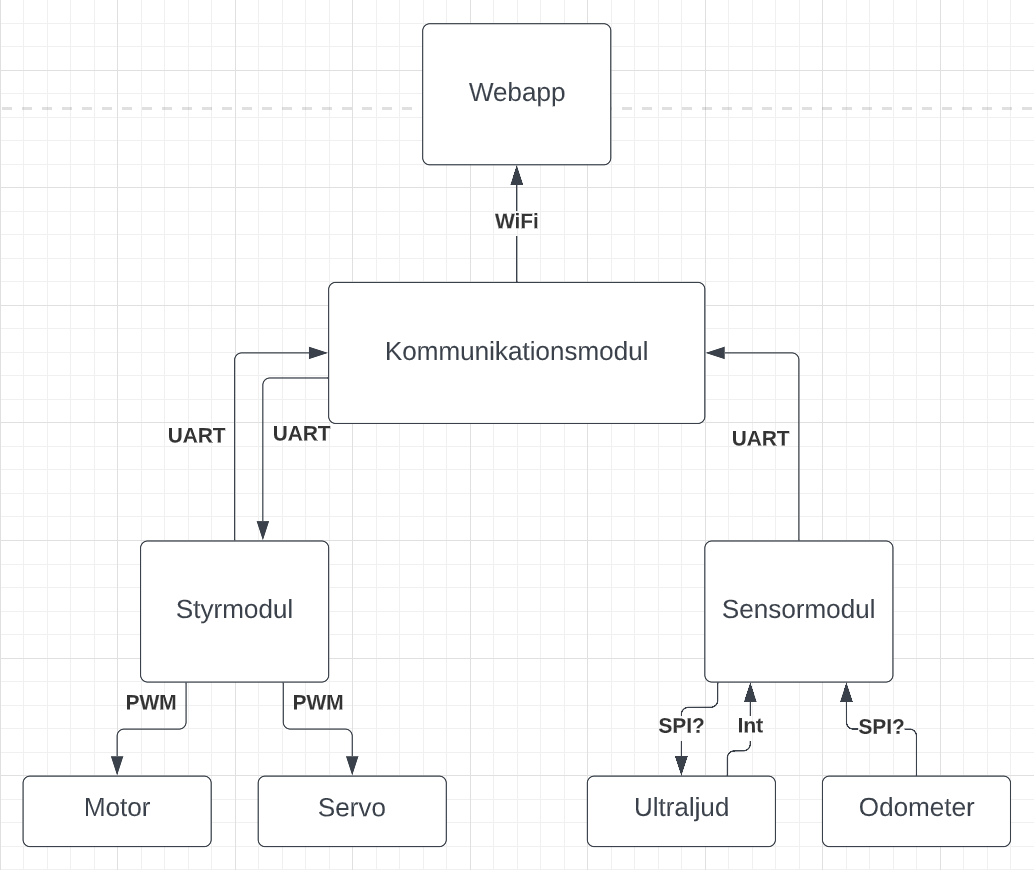
\includegraphics[width=.5\textwidth]{./Figures/blockskiss.png}
  \caption{Övergripande blockschema över systemet som ska konstrueras.}
  \label{fig:blockskiss}
\end{figure}

I figur \ref{fig:blockskiss} syns ett övergripande blockschema över systemet som ska konstrueras. Den visar de fyra delsystemen \emph{kommunikations-, styr-} och \emph{sensormodulerna} samt den \emph{externa applikationen}, i bilden benämnd ``Webapp``. I centrum står kommuikationsmodulen som är det enda delsystem som är anslutet direkt till dem andra delsystemen. All data som behöver nå en annan modul går alltid via kommunikationsmodulen först om datan inte redan kommer därifrån.
Kommunikationsmodulen är ansluten till både sensor- och styr-modulen via \emph{UART}-protokoll och till webappen via WiFi. De tre modulerna ska alla kunna bytas ut mot en annan modul som efterföljer protokollet för den modulen, även om projektet endast bidrar en av varje. 

\section{Datorseende}
Plan för datorseende är att ta emot bild från Raspberry-pi kameran, omvandla denna bild till gråskala och reducera brus, köra en algoritm för att markera ut mörka kanter, rita linjer längs med dessa kanter, passa en mask till dessa linjer, beräkna vinkel och skicka relevant information till styrmodul. Efter att vi har verifierat att detta fungerar så minskar vi upplösning och försöker få så bra prestanda som möjligt.


\section{Delsystem 1: Kommunikationsmodul}
Kommunikationsmodulen består av en Raspberry-pi 3B+ och en Raspberry-pi-kamera. Denna modul ansvarar för ett antal saker, för det första är modulen ansvarig för att bearbeta data som tas emot från kameran och skicka vidare till styrmodulen. 
Kommunikationsmodulen fungerar också som en brygga mellan sensormodulen och styrmodulen, den tar emot data från sensormodulen och skickar vidare till styrmodulen.
Utöver de ovan nämnda funktionerna skickar kommunikationsmodulen all tillgänglig data till en extern dator. Kommunikationsmodulen kan också ta emot kommandon från en extern enhet och vidarebefordra dessa till styrmodulen.

\section{Delsystem 2: Styrmodul}
Styrmodulen består av en ATmegaprocessor. Denna processor har i uppdrag att ta emot data från Rasberry-Pi och sedan bestämma hur mycket hjulen ska svänga (troligtvis med någon form av PD-reglering), gasa eller bromsa bilen. Den styr motorer och hjulaxeln genom ett antal kontrollsignaler som finns färdiga genom ett kontaktdon i bilens skelett. 



\begin{figure}[htbp]
  \centering
  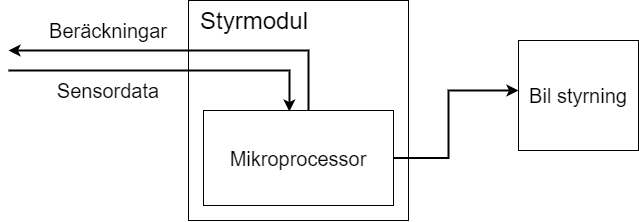
\includegraphics[width=.5\textwidth]{./Figures/styrmodul-projektskiss.png}
  \caption{Övergripande blockschema över styrmodulen.}
  \label{fig:styrmodul}
\end{figure}

\section{Delsystem 3: Sensormodul}
Sensormodulen består av en ATmegaprocessor, en ultraljudsensor, 2 halleffektssensorer. Sensormodulen samlar data från dessa sensorer, och skickar sedan vidare datan till kommunikationsmodulen.

\begin{figure}[htbp]
  \centering
  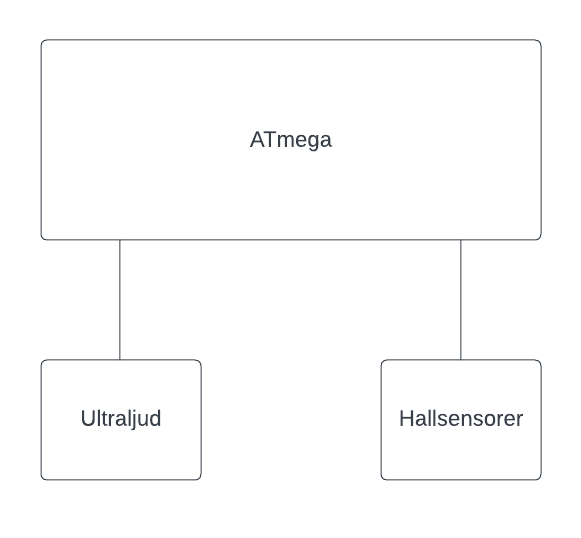
\includegraphics[width=.3\textwidth]{./Figures/Sensormodul.png}
  \caption{Väldigt enkel skiss på sensormodulen och de komponenter som är kopplade till den.}
  \label{fig:sensorskiss}
\end{figure}

\section{Delsystem 4: Extern Applikation}
\begin{figure}[htbp]
  \centering
  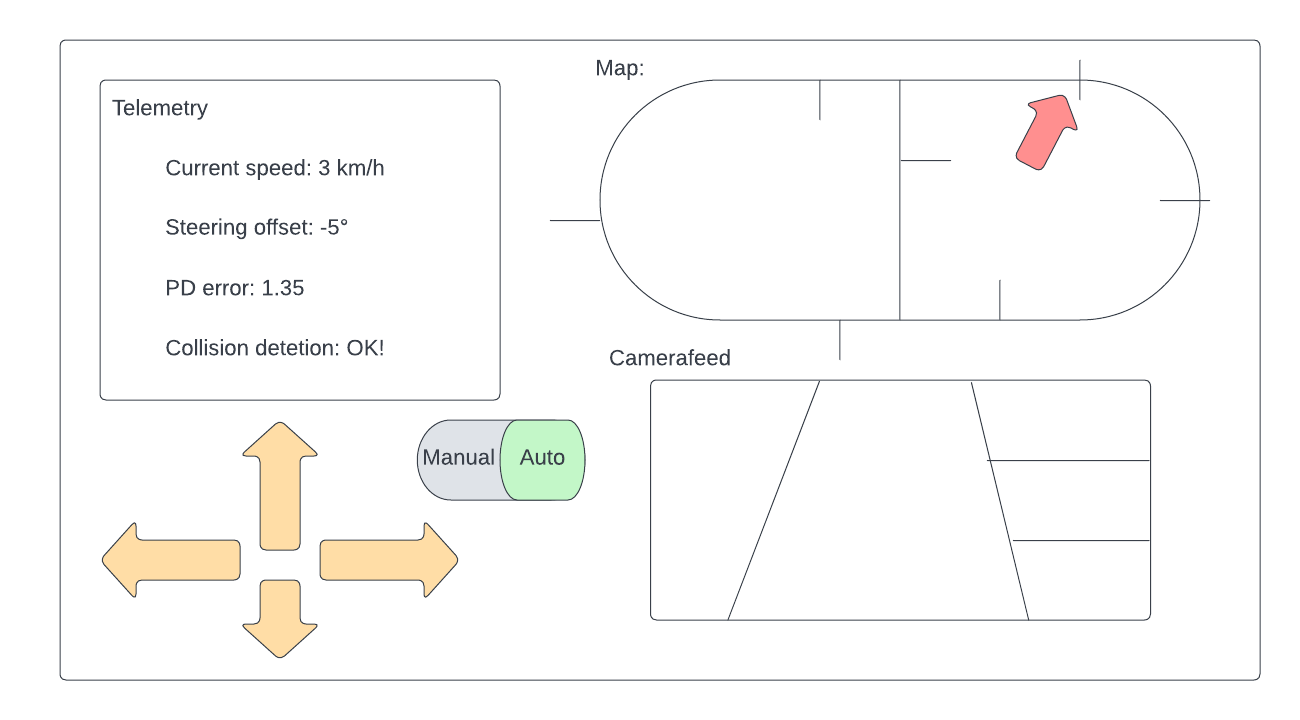
\includegraphics[width=.8\textwidth]{./Figures/appskiss.png}
  \caption{Väldigt enkel skiss på hur layouten på den externa applikationen skulle kunna se ut.}
  \label{fig:appskiss}
\end{figure}

Den Externa Applikationen består av en webserver (P2P) som körs på en dator och kommunicerar telemetri och eventuellt en videoström mellan kommunikationsenheten och applikationen. Telemetrin består av styrparametrar, som då kan ändra hur bilen beter sig på banan. 

Figur \ref{fig:appskiss} visar ett exempel på hur layouten på applikationen skulle kunna se ut. Det finns fält med information om diverse styrparametrar och sensordata. Det finns möjlighet att växla mellan autonomt och manuellt styrläge och knappar eller på något annat vis möjlighet att skicka manuella styrkommandon till taxibilen. Vid sidan om kan man se en visualisering av banan med bilens position och en separat ruta som visar livebilder från kameran. Lämpligtvis finns det även möjlighet att ange och starta ett autonomt köruppdrag. 


% \clearpage
% \bibliography{references}

\end{document}